\chapter{हरित रसायन और औद्योगिक प्रक्रम}\label{ch:b3:green-industrial}

आइबुप्रोफ़ेन पहले छह चरणों में बनाया जाता था जो जितना द्रव्यमान रखते थे उससे अधिक
फेंक देते थे: हर किलोग्राम औषध के लिए ऐलुमिनियम लवण, सोडियम क्लोराइड, एथेनॉल,
अमोनिया और ऐसीटिक अम्ल संयंत्र से बाहर जाते थे। 1992 से एक त्रि-चरणीय उत्प्रेरकी मार्ग
अपने प्रयुक्त अधिकांश परमाणुओं को उत्पाद में बदलता आया है, और उसका एकमात्र
उप-उत्पाद, ऐसीटिक अम्ल, पुनःप्राप्त करके बेचा जाता है। यह अध्याय ऐसी तुलनाओं को
संख्याएँ देता है: \omterm{def:b3:green-industrial:atom-economy}{परमाणु मितव्ययिता}, \omterm{def:b3:green-industrial:e-factor}{E-गुणक} और \omterm{def:b3:green-industrial:pmi}{प्रक्रम द्रव्यमान तीव्रता}; फिर यह
विलायकों, ऊर्जा और \omterm{def:b3:green-industrial:lca}{जीवन-चक्र मूल्यांकन} को देखता है, यह कि कुछ सबसे बड़े रासायनिक
प्रक्रमों को कैसे स्वच्छतर बनाया गया, और यह कि \omterm{def:b3:green-industrial:feedstock}{नवीकरणीय कच्चे माल} और
\omterm{def:b3:complex-kinetics:enzyme}{एंज़ाइम} क्या बदलते हैं।

\begin{recall}
विद्यालय के खंड ने \omterm{def:b3:green-industrial:atom-economy}{परमाणु मितव्ययिता} और \omterm{def:b3:green-industrial:green-chemistry}{हरित रसायन} प्रस्तुत किए; प्रथम वर्ष के
खंड ने लब्धियाँ; द्वितीय वर्ष के खंड ने रिएक्टर, रूपांतरण, वरणात्मकता, निवास
काल, एकल-पारण रूपांतरण, पुनश्चक्रण और निष्कासन, रुद्धोष्म ताप-वृद्धि,
विद्युत-अपघटक और ईंधन सेल। \Cref{ch:b3:surfaces-catalysis} और
\cref{ch:b3:homogeneous-catalysis} ने उत्प्रेरण का विवेचन किया,
\cref{ch:b3:total-synthesis} ने किसी संश्लेषी मार्ग के मापों का।
\end{recall}

\begin{omfigure}
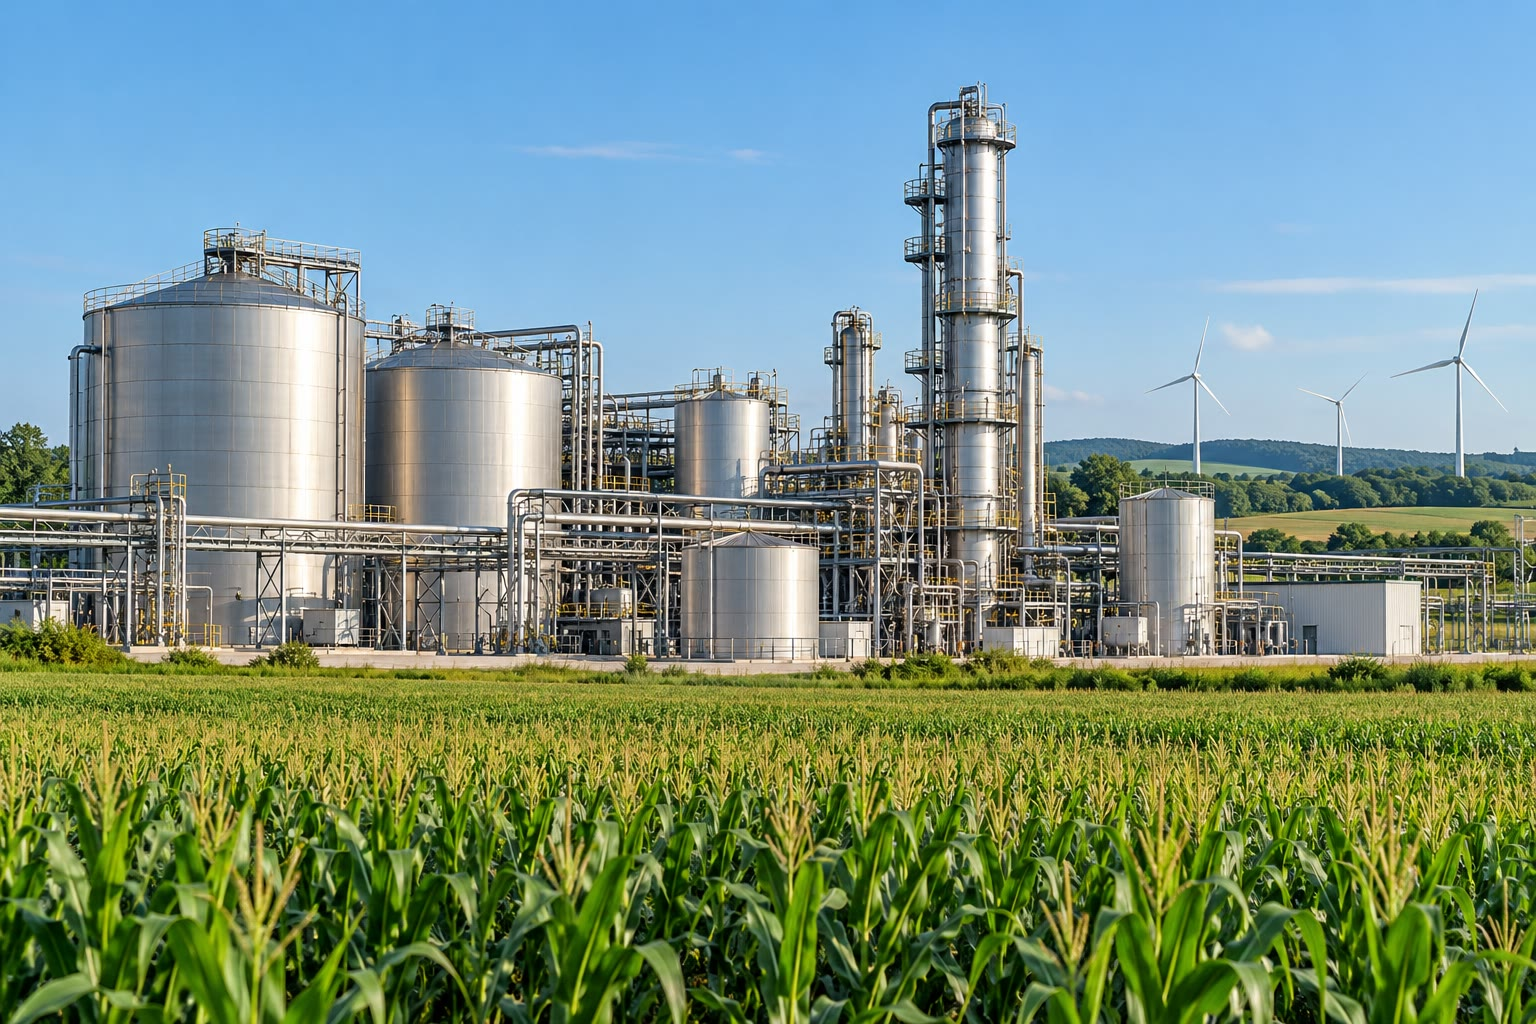
\includegraphics[width=0.58\linewidth]{images/book4/ai/b3-31-biorefinery.jpg}

{\small एक जैवशोधनशाला: किण्वन टंकियाँ और एक आसवन स्तंभ, जो
फ़सलों और अवशेषों को ईंधनों और प्लेटफ़ॉर्म रसायनों में बदलते हैं।}
\end{omfigure}

\section{हरितता को मापना}

\begin{definition}[हरित रसायन]\label{def:b3:green-industrial:green-chemistry}
\emph{हरित रसायन}\index{हरित रसायन} ऐसे रासायनिक
उत्पादों और प्रक्रमों की अभिकल्पना है जो ख़तरनाक पदार्थों के उपयोग और उत्पादन को
घटाते या समाप्त करते हैं, जिसका सार बारह सिद्धांतों में है: अपशिष्ट रोकिए, \omterm{def:b3:green-industrial:atom-economy}{परमाणु
मितव्ययिता} अधिकतम कीजिए, कम ख़तरनाक पदार्थ प्रयुक्त कीजिए और बनाइए, सुरक्षित उत्पाद अभिकल्पित कीजिए,
सुरक्षित विलायक प्रयुक्त कीजिए, ऊर्जा बचाइए, \omterm{def:b3:green-industrial:feedstock}{नवीकरणीय कच्चे माल} प्रयुक्त कीजिए, अनावश्यक
व्युत्पन्नों से बचिए, रससमीकरणमितीय अभिकर्मकों की अपेक्षा उत्प्रेरकों को वरीयता दीजिए, निम्नीकरण के लिए
अभिकल्पना कीजिए, वास्तविक समय में निगरानी कीजिए, और स्वभावतः सुरक्षित रसायन चुनिए।
\end{definition}

\begin{definition}[परमाणु मितव्ययिता]\label{def:b3:green-industrial:atom-economy}
किसी अभिक्रिया की \emph{परमाणु मितव्ययिता}\index{परमाणु मितव्ययिता} वांछित उत्पाद का
मोलर द्रव्यमान है, संतुलित समीकरण के सभी अभिकारकों के मोलर द्रव्यमानों के
योग से भाग देकर, प्रतिशत के रूप में।
\end{definition}

\begin{proposition}[अभिक्रिया-वर्ग के अनुसार परमाणु मितव्ययिता]\label{prop:b3:green-industrial:ae-classes}
योगों और पुनर्विन्यासों की \omterm{def:b3:green-industrial:atom-economy}{परमाणु मितव्ययिता} 100\,\% होती है; प्रतिस्थापनों और
विलोपनों की कम।
\end{proposition}

\begin{proof}
किसी योग, $\mathrm{A} + \mathrm{B} \to \mathrm{AB}$, या पुनर्विन्यास, $\mathrm{A} \to \mathrm{A'}$, में एकमात्र उत्पाद अभिकारकों के सभी
परमाणु रखता है, अतः उसका मोलर द्रव्यमान उनके मोलर द्रव्यमानों के योग के बराबर होता है। कोई
प्रतिस्थापन, $\mathrm{A{-}X} + \mathrm{Y} \to \mathrm{A{-}Y} + \mathrm{X}$, या विलोपन, $\mathrm{A} \to \mathrm{B} + \mathrm{C}$, एक
दूसरा उत्पाद देता है जो द्रव्यमान को बाहर ले जाता है।
\end{proof}

\begin{definition}[E-गुणक]\label{def:b3:green-industrial:e-factor}
किसी प्रक्रम का \emph{E-गुणक}\index{E-गुणक} प्रति उत्पाद-द्रव्यमान अपशिष्ट का
द्रव्यमान है। पूर्ण E-गुणक में वे सभी निवेश जो उत्पाद में नहीं पहुँचते, अपशिष्ट
गिने जाते हैं, विलायक और जल सहित; सरल E-गुणक विलायकों और
जल को छोड़ देता है।
\end{definition}

\begin{definition}[प्रक्रम द्रव्यमान तीव्रता]\label{def:b3:green-industrial:pmi}
\emph{प्रक्रम द्रव्यमान तीव्रता}\index{प्रक्रम द्रव्यमान तीव्रता} (PMI) किसी
प्रक्रम में डाले गए पदार्थों (अभिकारक, अभिकर्मक, विलायक,
जल) का कुल द्रव्यमान है, प्रति उत्पाद-द्रव्यमान।
\end{definition}

\begin{proposition}[PMI और E-गुणक]\label{prop:b3:green-industrial:pmi-e}
समान परिसीमा के लिए $\mathrm{PMI} = E + 1$, जहाँ $E$ पूर्ण \omterm{def:b3:green-industrial:e-factor}{E-गुणक} है।
\end{proposition}

\begin{proof}
द्रव्यमान संरक्षण से, जो कुछ डाला जाता है वह या तो उत्पाद के रूप में या अपशिष्ट के रूप में निकलता है:
$m_{\text{प्रविष्ट}} = m_{\text{उत्पाद}} + m_{\text{अपशिष्ट}}$। $m_{\text{उत्पाद}}$ से भाग देने पर $\mathrm{PMI} = 1 + E$ मिलता है।
\end{proof}

\begin{definition}[अभिक्रिया द्रव्यमान दक्षता]\label{def:b3:green-industrial:rme}
किसी अभिक्रिया की \emph{अभिक्रिया द्रव्यमान दक्षता}\index{अभिक्रिया द्रव्यमान दक्षता} (RME)
प्राप्त उत्पाद का द्रव्यमान है, प्रयुक्त अभिकारकों के कुल द्रव्यमान से
भाग देकर।
\end{definition}

\begin{proposition}[लब्धि और परमाणु मितव्ययिता से RME]\label{prop:b3:green-industrial:rme}
$\mathrm{RME} = \mathrm{AE} \times \text{लब्धि}/\mathrm{SF}$, जहाँ रससमीकरणमितीय गुणक $\mathrm{SF} \ge 1$ प्रयुक्त अभिकारकों का
द्रव्यमान है, संतुलित समीकरण द्वारा अपेक्षित द्रव्यमान से भाग देकर।
\end{proposition}

\begin{proof}
अपेक्षित उत्पाद के एक मोल के लिए समीकरण को अभिकारकों का $\sum M_r$ द्रव्यमान चाहिए और
प्रयोग $\mathrm{SF}\sum M_r$ प्रयुक्त करता है; यह $\text{लब्धि} \times M_{\mathrm p}$ उत्पाद देता है। भाग देने पर:
$\mathrm{RME} = \text{लब्धि}\,M_{\mathrm p}/(\mathrm{SF}\sum M_r) = \mathrm{AE} \times \text{लब्धि}/\mathrm{SF}$।
\end{proof}

\begin{method}[किसी मार्ग के मापदंडों का परिकलन]\label{met:b3:green-industrial:metrics}
\begin{enumerate}
  \item प्रत्येक चरण का संतुलित समीकरण लिखिए और मार्ग में प्रवेश करने वाले सभी
        अभिकारकों से मार्ग की \omterm{def:b3:green-industrial:atom-economy}{परमाणु मितव्ययिता} परिकलित कीजिए।
  \item बैच अभिलेख से, डाली गई हर चीज़ के द्रव्यमान जोड़िए (अभिकारक,
        अभिकर्मक, विलायक, जल, उपचार-पश्चात् प्रक्रिया के पदार्थ): PMI = कुल निवेश / उत्पाद।
  \item $E = \mathrm{PMI} - 1$; यदि पुनःप्राप्त और पुनःप्रयुक्त धाराएँ परिसीमा के भीतर हों तो उन्हें
        घटाइए, और यह स्पष्ट बताइए।
  \item प्रत्येक चरण के लिए RME: उत्पाद / अभिकारक, यह पता लगाने के लिए कि पदार्थ कहाँ खोता है
        (कम लब्धि, अधिक अभिकर्मक, या ख़राब \omterm{def:b3:green-industrial:atom-economy}{परमाणु मितव्ययिता})।
\end{enumerate}
\end{method}

\begin{omfigure}
\begin{tikzpicture}
\begin{axis}[name=a, width=0.48\linewidth, height=5.4cm, ybar, bar width=14pt, ymin=0, ymax=110,
  xtick={1,2,3,4}, xticklabels={{आइबुप्रोफ़ेन, 6 चरण}, {आइबुप्रोफ़ेन, 3 चरण}, {EO, क्लोरोहाइड्रिन}, {EO, प्रत्यक्ष}},
  x tick label style={font=\scriptsize, rotate=25, anchor=north east}, ylabel={परमाणु मितव्ययिता / \%},
  axis lines=left, tick label style={font=\scriptsize}, label style={font=\small},
  nodes near coords, nodes near coords style={font=\scriptsize, /pgf/number format/fixed, /pgf/number format/precision=0},
  enlarge x limits=0.18]
\addplot[fill=omMeth!55, draw=omMeth] table[x=i, y=AE] {figdata/out/bachelor-3-green-metrics.dat};
\end{axis}
\begin{axis}[at={(a.east)}, anchor=west, xshift=1.4cm, width=0.48\linewidth, height=5.4cm, ybar, bar width=14pt, ymin=0, ymax=3.4,
  xtick={1,2,3,4}, xticklabels={{आइबुप्रोफ़ेन, 6 चरण}, {आइबुप्रोफ़ेन, 3 चरण}, {EO, क्लोरोहाइड्रिन}, {EO, प्रत्यक्ष}},
  x tick label style={font=\scriptsize, rotate=25, anchor=north east}, ylabel={न्यूनतम E-गुणक},
  axis lines=left, tick label style={font=\scriptsize}, label style={font=\small},
  nodes near coords, nodes near coords style={font=\scriptsize, /pgf/number format/fixed, /pgf/number format/precision=2},
  enlarge x limits=0.18]
\addplot[fill=omThm!45, draw=omThm] table[x=i, y=Emin] {figdata/out/bachelor-3-green-metrics.dat};
\end{axis}
\end{tikzpicture}

{\small आइबुप्रोफ़ेन तक के दो मार्गों और एथिलीन ऑक्साइड (EO) तक के दो मार्गों की
\omterm{def:b3:green-industrial:atom-economy}{परमाणु मितव्ययिताएँ}, और वे सबसे छोटे \omterm{def:b3:green-industrial:e-factor}{E-गुणक} जिनकी वे अनुमति देते हैं (सभी लब्धियाँ 100\,\%, कोई विलायक नहीं):
$E_{\min} = (1 - \mathrm{AE})/\mathrm{AE}$। वास्तविक \omterm{def:b3:green-industrial:e-factor}{E-गुणक}, 100\,\% से कम लब्धियों, अधिक अभिकर्मकों और
विलायकों के साथ, बड़े होते हैं।}
\end{omfigure}

\section{विलायक और ऊर्जा}

किसी सूक्ष्म-रसायन या औषधीय प्रक्रम के द्रव्यमान का सबसे बड़ा भाग प्रायः विलायक
होते हैं। विलायक चयन मार्गदर्शिकाएँ उन्हें सुरक्षा, स्वास्थ्य और
पर्यावरणीय मानदंडों पर श्रेणीबद्ध करती हैं: जल, एथेनॉल, एथिल ऐसीटेट, 2-मेथिलटेट्राहाइड्रोफ़्यूरान
और ऐनिसोल अनुशंसित हैं; डाइक्लोरोमेथेन, क्लोरोफ़ॉर्म, बेंज़ीन, हेक्सेन,
डाइमेथिलफ़ॉर्मामाइड और 1,4-डाइऑक्सेन से बचना चाहिए या वे प्रतिबंधित हैं। जल,
अतिक्रांतिक कार्बन डाइऑक्साइड (जो अध्रुवीय यौगिकों को घोलती है और दाब हटाने पर
कोई अवशेष नहीं छोड़ती) और विलायक-मुक्त अभिक्रियाएँ समस्या को उसके
स्रोत पर ही हटा देती हैं।

\begin{method}[विलायक चयन मार्गदर्शिका का उपयोग]\label{met:b3:green-industrial:solvent-choice}
\begin{enumerate}
  \item सूचीबद्ध कीजिए कि विलायक को क्या करना है: अभिकारकों को घोलना, अभिकर्मकों के साथ टिके रहना,
        उपयोगी ताप पर उबलना, उपचार-पश्चात् प्रक्रिया में जल से अलग होना।
  \item पहले अनुशंसित वर्ग से चुनिए; उसके संकट-कथन जाँचिए।
  \item यदि कोई समस्याजनक विलायक आवश्यक हो, तो समान कार्य वाला कोई अनुशंसित विलायक
        खोजिए (निष्कर्षणों में डाइक्लोरोमेथेन या THF के स्थान पर
        2-मेथिलटेट्राहाइड्रोफ़्यूरान, वर्णलेखन में हेक्सेन के स्थान पर एथिल ऐसीटेट और हेप्टेन)।
  \item आसवन द्वारा उसकी पुनःप्राप्ति की योजना बनाइए, और जो खोता है उसे \omterm{def:b3:green-industrial:e-factor}{E-गुणक} में गिनिए।
\end{enumerate}
\end{method}

\begin{definition}[प्रक्रम गहनीकरण]\label{def:b3:green-industrial:intensification}
\emph{प्रक्रम गहनीकरण}\index{प्रक्रम गहनीकरण} उपकरण और संचालन
परिस्थितियों की ऐसी पुनर्अभिकल्पना है जो किसी प्रक्रम को कहीं छोटा,
सुरक्षित या अधिक दक्ष बना दे: छोटे आयतनों और
बड़े ऊष्मा-विनिमय क्षेत्रफलों वाले सतत प्रवाह रिएक्टर, अभिक्रियाशील आसवन, माइक्रोवेव तापन।
\end{definition}

प्रवाह रिएक्टर में किसी भी क्षण किसी संकटपूर्ण मध्यवर्ती का केवल छोटा आयतन
विद्यमान होता है, और ऊष्मा किसी बड़े बैच पात्र की तुलना में कहीं तेज़ी से हटाई जाती है; जो अभिक्रियाएँ
किसी टंकी में अनियंत्रित हो जातीं, उन्हें ऊँचे तापों और
सांद्रताओं पर चलाया जा सकता है। उत्प्रेरक रससमीकरणमितीय अभिकर्मकों का स्थान लेते हैं, जिससे
अभिकर्मक और उससे बनने वाला अपशिष्ट दोनों बचते हैं: पुराने
आइबुप्रोफ़ेन मार्ग का फ़्रीडेल--क्राफ़्ट्स ऐसिलन रससमीकरणमितीय मात्रा में ऐलुमिनियम क्लोराइड प्रयुक्त करता था, जो
उपचार-पश्चात् प्रक्रिया में नष्ट हो जाता था; नया मार्ग हाइड्रोजन फ़्लुओराइड को उत्प्रेरक और विलायक दोनों के रूप में प्रयुक्त करता है,
जिसे पुनःप्राप्त और पुनःप्रयुक्त किया जाता है।

\section{जीवन-चक्र दृष्टि}

\begin{definition}[जीवन-चक्र मूल्यांकन]\label{def:b3:green-industrial:lca}
\emph{जीवन-चक्र मूल्यांकन}\index{जीवन-चक्र मूल्यांकन} (LCA) किसी उत्पाद के
उसके पूरे जीवन में, कच्चे माल के निष्कर्षण से निपटान तक, पर्यावरणीय प्रभावों का मूल्यांकन
करता है। इसे \emph{क्रियात्मक इकाई}\index{क्रियात्मक इकाई} के प्रति व्यक्त किया जाता है,
अर्थात् प्रदान की गई सेवा (उदाहरण के लिए, कपड़ों के एक भार की एक धुलाई), एक
\emph{निकाय परिसीमा}\index{निकाय परिसीमा} के भीतर जो बताती है कि कौन-से प्रक्रम
सम्मिलित हैं। \emph{पालने-से-द्वार मूल्यांकन}\index{पालने-से-द्वार मूल्यांकन}
उत्पाद के कारख़ाने से निकलते ही रुक जाता है।
\end{definition}

\begin{omfigure}
\begin{tikzpicture}[font=\scriptsize, >=Stealth,
  box/.style={draw, rounded corners, fill=omDef!10, align=center, minimum height=8mm, inner sep=3pt}]
  \node[box] (r) at (0,0) {कच्चे माल का\\ निष्कर्षण};
  \node[box] (p) at (2.6,0) {रासायनिक\\ उत्पादन};
  \node[box] (f) at (5.2,0) {सूत्रण,\\ पैकेजिंग};
  \node[box] (u) at (7.8,0) {उपयोग};
  \node[box] (e) at (10.2,0) {जीवन का अंत:\\ पुनर्चक्रण, निपटान};
  \foreach \a/\b in {r/p, p/f, f/u, u/e} \draw[->, thick] (\a) -- (\b);
  \draw[omThm, thick, dashed, rounded corners] (-1.1,-0.75) rectangle (3.75,0.75);
  \node[omThm, anchor=north] at (1.3,-0.8) {पालने-से-द्वार परिसीमा};
  \draw[omMeth, thick, dashed, rounded corners] (-1.25,-1.35) rectangle (11.5,0.95);
  \node[omMeth, anchor=north] at (5.1,-1.4) {पालने-से-कब्र परिसीमा};
  \node[anchor=south] at (5.1,1.0) {निवेश: पदार्थ, ऊर्जा, जल \quad निर्गम: उत्पाद, उत्सर्जन, अपशिष्ट};
\end{tikzpicture}

{\small किसी उत्पाद के जीवन के चरण और दो निकाय परिसीमाएँ। परिसीमा के भीतर प्रत्येक
प्रक्रम के निवेशों और निर्गमों की सूची बनाई जाती है और उन्हें प्रति \omterm{def:b3:green-industrial:lca}{क्रियात्मक इकाई}
प्रभाव-श्रेणियों (जलवायु परिवर्तन, अम्लीकरण, जल-उपयोग, विषाक्तता\dots) में
बदला जाता है।}
\end{omfigure}

\begin{definition}[कार्बन पदचिह्न]\label{def:b3:green-industrial:carbon-footprint}
किसी उत्पाद का \emph{कार्बन पदचिह्न}\index{कार्बन पदचिह्न} उसका
जीवन-चक्र ग्रीनहाउस गैस उत्सर्जन है, जिसे उतने ही तापन प्रभाव वाली
कार्बन डाइऑक्साइड के द्रव्यमान के रूप में व्यक्त किया जाता है।
\end{definition}

\begin{method}[तुलनात्मक LCA की स्थापना]\label{met:b3:green-industrial:lca}
\begin{enumerate}
  \item लक्ष्य और \omterm{def:b3:green-industrial:lca}{क्रियात्मक इकाई} बताइए: उसकी तुलना कीजिए जो समान
        सेवा देता है, समान द्रव्यमान नहीं।
  \item दोनों विकल्पों के लिए एक ही \omterm{def:b3:green-industrial:lca}{निकाय परिसीमा} खींचिए।
  \item उसके भीतर प्रत्येक प्रक्रम के निवेशों और निर्गमों की सूची बनाइए, आँकड़ों के
        स्रोतों और तिथियों के साथ।
  \item प्रभाव-श्रेणियों में बदलिए, फिर समझौतों (कम कार्बन पर
        अधिक जल) को खोजिए और परखिए कि निष्कर्ष आँकड़ों के प्रति कितना संवेदनशील है।
\end{enumerate}
\end{method}

\section{प्रमुख प्रक्रम और उनका सुधार}

\begin{proposition}[अमोनिया से कार्बन डाइऑक्साइड]\label{prop:b3:green-industrial:smr}
मेथेन के भाप-रिफ़ॉर्मिंग से प्राप्त हाइड्रोजन से अमोनिया बनाने पर, केवल
कच्चे माल से ही, $3/8$ मोल $\ce{CO2}$ प्रति मोल $\ce{NH3}$ मुक्त होता है: लगभग \qty{0.97}{t} $\ce{CO2}$ प्रति टन अमोनिया।
\end{proposition}

\begin{proof}
रिफ़ॉर्मिंग और उसके बाद जल--गैस विस्थापन मिलकर $\ce{CH4 + 2H2O -> CO2 + 4H2}$ है। संश्लेषण
$\ce{N2 + 3H2 -> 2NH3}$ है: अमोनिया के दो मोलों को हाइड्रोजन के तीन चाहिए, अर्थात् $3/4$ मोल
मेथेन और $3/4$ मोल $\ce{CO2}$; अमोनिया के प्रति मोल, $3/8$। एक टन अमोनिया
(\qty{17.0}{g/mol}) $\qty{5.88e4}{mol}$ है, जिससे $\qty{2.21e4}{mol} \times \qty{44.0}{g/mol} = \qty{0.97}{t}$ $\ce{CO2}$ मिलता है। रिफ़ॉर्मिंग की ऊष्मा के लिए
मेथेन जलाने से और अधिक जुड़ता है।
\end{proof}

% ledger: nh3:world-2024
अमोनिया संयंत्र, जो प्रति वर्ष लगभग 15 करोड़ टन नाइट्रोजन बनाते हैं, औद्योगिक
कार्बन डाइऑक्साइड के सबसे बड़े एकल स्रोतों में हैं; निम्न-कार्बन बिजली से
विद्युत-अपघटन द्वारा हाइड्रोजन, या रिफ़ॉर्मर पर कार्बन प्रग्रहण,
इसे घटाने के मार्ग हैं। स्वयं अमोनिया पाश, अपने कम एकल-पारण
रूपांतरण, अरूपांतरित गैस के पुनश्चक्रण और उस आर्गन और मेथेन के निष्कासन के साथ जो
अन्यथा संचित हो जाते, पहले से ही दक्ष है।

\begin{omfigure}
\begin{tikzpicture}[font=\scriptsize, >=Stealth,
  box/.style={draw, rounded corners, fill=omMeth!10, align=center, minimum height=8mm, inner sep=3pt}]
  \node[box] (m) at (0,0) {मिश्रक};
  \node[box] (c) at (2.6,0) {संपीडक};
  \node[box] (r) at (5.2,0) {परिवर्तक\\ (आयरन उत्प्रेरक)};
  \node[box] (s) at (8.0,0) {संघनित्र,\\ पृथक्कारी};
  \draw[->, thick] (-1.8,0) -- (m) node[pos=0, left, align=right] {$\ce{N2 + 3H2}$\\ (पूरक)};
  \draw[->, thick] (m) -- (c); \draw[->, thick] (c) -- (r); \draw[->, thick] (r) -- (s);
  \draw[->, thick] (s) -- ++(0,-1.2) node[below] {द्रव $\ce{NH3}$};
  \draw[->, thick] (s.north) -- ++(0,0.8) -| node[pos=0.25, above] {अरूपांतरित गैस का पुनश्चक्रण} (m.north);
  \draw[->, thick, omThm] ($(s.north)+(0,0.8)$) -- ++(1.6,0) node[right] {निष्कासन (Ar, $\ce{CH4}$)};
\end{tikzpicture}

{\small अमोनिया संश्लेषण पाश: ताज़ी गैस पुनश्चक्रित गैस के साथ मिलाई जाती है,
संपीडित की जाती है और उत्प्रेरक के ऊपर से गुज़ारी जाती है; अमोनिया संघनित करके निकाल ली जाती है, अरूपांतरित
गैस लौटती है, और एक छोटी निष्कासन धारा उन अक्रिय गैसों को हटाती है जो
अन्यथा जमा हो जातीं।}
\end{omfigure}

अन्य बड़े प्रक्रम भी यही सीख देते हैं। सल्फ़्यूरिक
अम्ल का संपर्क प्रक्रम इतना ऊष्माक्षेपी है कि आधुनिक संयंत्र भाप और बिजली का निर्यात करता है।
एथिलीन ऑक्साइड पहले एथिलीन क्लोरोहाइड्रिन के माध्यम से बनाया जाता था, कैल्सियम
क्लोराइड अपशिष्ट के साथ; सिल्वर पर ऑक्सीजन से एथिलीन के प्रत्यक्ष ऑक्सीकरण ने, जो
100\,\% \omterm{def:b3:green-industrial:atom-economy}{परमाणु मितव्ययिता} वाला एक योग है, उसका स्थान लिया, कुछ एथिलीन के
कार्बन डाइऑक्साइड में जल जाने की कीमत पर। प्रोपिलीन ऑक्साइड अब टाइटेनियम \omterm{def:b3:inorganic-materials:zeolite}{ज़िओलाइट}
उत्प्रेरक पर हाइड्रोजन पेरॉक्साइड से भी बनाया जाता है, जिसमें जल ही एकमात्र उप-उत्पाद है। ऐडिपिक अम्ल,
जो साइक्लोहेक्सेनॉल और साइक्लोहेक्सेनोन को नाइट्रिक अम्ल से ऑक्सीकृत करके बनाया जाता है, नाइट्रस
ऑक्साइड मुक्त करता है, एक प्रबल ग्रीनहाउस गैस, जिसे संयंत्र अब उत्प्रेरकी रूप से नष्ट करते हैं।

\section{नवीकरणीय कच्चे माल और जैवउत्प्रेरण}

\begin{definition}[नवीकरणीय कच्चे माल]\label{def:b3:green-industrial:feedstock}
\emph{नवीकरणीय कच्चा माल}\index{नवीकरणीय कच्चा माल} ऐसा कच्चा माल है जिसकी
पूर्ति मानवीय समय-पैमाने पर हो जाती है, जैसे पादप जैवभार। \emph{प्लेटफ़ॉर्म
अणु}\index{प्लेटफ़ॉर्म अणु} उससे बड़ी मात्रा में बनाया गया एक सरल यौगिक है जिसे
अनेक उत्पादों में बदला जाता है: एथेनॉल, लैक्टिक अम्ल, सक्सिनिक अम्ल,
ग्लिसरॉल, लेवुलिनिक अम्ल, फ़रफ़्यूरल, 5-(हाइड्रॉक्सीमेथिल)फ़रफ़्यूरल।
\end{definition}

\begin{definition}[जैवउत्प्रेरण]\label{def:b3:green-industrial:biocatalysis}
\emph{जैवउत्प्रेरण}\index{जैवउत्प्रेरण} \omterm{def:b3:complex-kinetics:enzyme}{एंज़ाइमों} का, पृथक रूप में या
कोशिकाओं के भीतर, रासायनिक रूपांतरणों के उत्प्रेरकों के रूप में उपयोग है।
\end{definition}

\omterm{def:b3:complex-kinetics:enzyme}{एंज़ाइम} जल में कक्ष ताप के निकट उत्कृष्ट वरणात्मकता के साथ कार्य करते हैं, और
निर्देशित विकास अब उन्हें अप्राकृतिक क्रियाधारों के अनुरूप ढालता है: इसी उद्देश्य से
विकसित एक ट्रांसऐमिनेज़ ने मधुमेह की औषध सिटाग्लिप्टिन के निर्माण में
रोडियम-उत्प्रेरित असममित हाइड्रोजनन का स्थान लिया, और कीटोरिडक्टेज़ अनेक
किरैल ऐल्कोहॉल बनाते हैं। कार्बन डाइऑक्साइड स्वयं एक कच्चा माल है: यूरिया इससे और
अमोनिया से बनता है, और मेथेनॉल इससे और हाइड्रोजन से। पॉलिएथिलीन टेरेफ़्थैलेट को
ग्लाइकॉल-अपघटन या मेथेनॉल-अपघटन द्वारा, या अभियांत्रिकी द्वारा रूपांतरित
\omterm{def:b3:complex-kinetics:enzyme}{एंज़ाइमों} द्वारा, वापस उसके एकलकों में विबहुलकित करके फिर से बहुलकित किया जा सकता है।

\begin{inthelab}[उपचार-पश्चात् प्रक्रिया में डाइक्लोरोमेथेन का प्रतिस्थापन]
जिस उत्पाद को जल से डाइक्लोरोमेथेन द्वारा निष्कर्षित किया जाता था, उसे इसके स्थान पर
2-मेथिलटेट्राहाइड्रोफ़्यूरान से निष्कर्षित किया जाता है: यह जैवभार से बनता है, जल से
साफ़ अलग होता है (यह केवल आंशिक रूप से मिश्रणीय है), और ऊपरी परत है,
निचली नहीं, जिससे पृथक्कारी कीप की संक्रियाओं का क्रम बदल जाता है। कार्बनिक
परतों को शुष्क किया जाता है, विलायक को कम दाब पर आसवित करके हटाया और
पुनः उपयोग के लिए एकत्र किया जाता है।
\end{inthelab}

\begin{safety}{\ghs[0.62cm]{GHS02}\ghs[0.62cm]{GHS04}\ghs[0.62cm]{GHS06}\ghs[0.62cm]{GHS08}}
% ledger: ghs4:EO, ghs:CH2Cl2, ghs4:2MeTHF
एथिलीन ऑक्साइड: दाब में अत्यंत ज्वलनशील गैस, साँस में लेने पर विषैली, कैंसर
और आनुवंशिक दोष उत्पन्न कर सकती है; यह केवल बंद औद्योगिक तंत्रों
और जीवाणुरहितीकरण इकाइयों में ही विद्यमान होती है। डाइक्लोरोमेथेन एक संदिग्ध कैंसरजन है, और
2-मेथिलटेट्राहाइड्रोफ़्यूरान ज्वलनशील है और आँखों के लिए संक्षारक: हरित विलायक
हानिरहित विलायक नहीं होता।
\end{safety}

\begin{history}[बारह सिद्धांत और एक संख्या]
पॉल अनास्तास और जॉन वॉर्नर ने 1998 में \omterm{def:b3:green-industrial:green-chemistry}{हरित रसायन} के बारह सिद्धांत
प्रकाशित किए। रोजर शेल्डन ने 1992 में \omterm{def:b3:green-industrial:e-factor}{E-गुणक} प्रस्तुत किया, यह देखते हुए कि
सूक्ष्म-रसायन और औषध उद्योग, टन-भार में छोटे होते हुए भी,
थोक रसायन की तुलना में प्रति किलोग्राम उत्पाद कहीं अधिक अपशिष्ट उत्पन्न करते थे। 1992 में
आरंभ हुआ त्रि-चरणीय आइबुप्रोफ़ेन प्रक्रम इस नए दृष्टिकोण के
आरंभिक उदाहरणों में से एक बना।
\end{history}

\section{अभ्यास}

\begin{exercise}[$\star$]\label{exo:b3:green-industrial:1}
ब्यूटाडाईन की एथीन के साथ डील्स--ऐल्डर अभिक्रिया की, ऐसीटिक अम्ल के एथेनॉल के साथ
एस्टरीकरण की, और बेंज़ैल्डिहाइड की $\ce{Ph3P=CH2}$ के साथ विटिग अभिक्रिया की (जो स्टाइरीन और
ट्राइफ़ेनिलफ़ॉस्फ़ीन ऑक्साइड देती है) \omterm{def:b3:green-industrial:atom-economy}{परमाणु मितव्ययिता} परिकलित कीजिए।
\end{exercise}

\begin{exercise}[$\star$]\label{exo:b3:green-industrial:2}
एक बैच 120 kg पदार्थ (अभिकारक, विलायक और जल) प्रयुक्त करता है और 8.0 kg
उत्पाद देता है। PMI और पूर्ण \omterm{def:b3:green-industrial:e-factor}{E-गुणक} परिकलित कीजिए।
\end{exercise}

\begin{exercise}[$\star$]\label{exo:b3:green-industrial:3}
कपड़े धोने के दो डिटर्जेंटों की तुलना के लिए एक \omterm{def:b3:green-industrial:lca}{क्रियात्मक इकाई} चुनिए, और बताइए कि
``एक किलोग्राम पाउडर'' एक ख़राब विकल्प क्यों होता।
\end{exercise}

\begin{exercise}[$\star$]\label{exo:b3:green-industrial:4}
निष्कर्षण में डाइक्लोरोमेथेन, वर्णलेखन में हेक्सेन, और ऐमाइड युग्मन में DMF के
लिए हरित प्रतिस्थापन सुझाइए।
\end{exercise}

\begin{exercise}[$\star\star$]\label{exo:b3:green-industrial:5}
60.0 g ऐसीटिक अम्ल का 92.0 g एथेनॉल (रससमीकरणमितीय मात्रा का
दोगुना) के साथ एस्टरीकरण 70.4 g एथिल ऐसीटेट देता है। लब्धि, \omterm{def:b3:green-industrial:atom-economy}{परमाणु
मितव्ययिता}, रससमीकरणमितीय गुणक और RME परिकलित कीजिए, और उनके बीच का संबंध
जाँचिए।
\end{exercise}

\begin{exercise}[$\star\star$]\label{exo:b3:green-industrial:6}
एथिलीन ऑक्साइड तक के क्लोरोहाइड्रिन और प्रत्यक्ष-ऑक्सीकरण मार्गों की \omterm{def:b3:green-industrial:atom-economy}{परमाणु मितव्ययिताएँ}
परिकलित कीजिए, और पहले मार्ग द्वारा प्रति टन एथिलीन ऑक्साइड बनने वाले कैल्सियम क्लोराइड
का द्रव्यमान।
\end{exercise}

\begin{exercise}[$\star\star$]\label{exo:b3:green-industrial:7}
अध्याय के प्रति टन अमोनिया $\ce{CO2}$ की जाँच कीजिए, और भाप-रिफ़ॉर्मिंग द्वारा बने
हाइड्रोजन के प्रति टन $\ce{CO2}$ परिकलित कीजिए।
\end{exercise}

\begin{exercise}[$\star\star$]\label{exo:b3:green-industrial:8}
\qty{25}{\celsius} पर द्रव जल के विद्युत-अपघटन द्वारा एक किलोग्राम हाइड्रोजन बनाने के लिए न्यूनतम
विद्युत ऊर्जा, kWh में, $\Delta_rG^\circ$ से परिकलित कीजिए, और $\Delta_rH^\circ$ से ऊर्जा।
\end{exercise}

\begin{exercise}[$\star\star$]\label{exo:b3:green-industrial:9}
यदि एक मोल $\ce{N2O}$ ऐडिपिक अम्ल ($\ce{C6H10O4}$) के प्रति मोल बनता है और $\ce{N2O}$ की वैश्विक तापन
क्षमता 273 है (अभ्यास के आँकड़े), तो उपशमन के बिना प्रति टन ऐडिपिक अम्ल $\ce{N2O}$ और $\ce{CO2}$ तुल्यांक
परिकलित कीजिए।
\end{exercise}

\begin{exercise}[$\star\star\star$]\label{exo:b3:green-industrial:10}
दिखाइए कि जब अधिक अभिकर्मकों का पुनश्चक्रण किया जाता है, तो चरणों के अनुक्रम का समग्र RME
चरणों के RME का गुणनफल नहीं होता, और समझाइए कि पुनश्चक्रण
\omterm{def:b3:green-industrial:e-factor}{E-गुणक} को कैसे बदलता है।
\end{exercise}

\begin{exercise}[$\star\star\star$]\label{exo:b3:green-industrial:11}
एक प्रक्रम-सुधार किसी चरण में विलायक को प्रति किलोग्राम उत्पाद 20 L से घटाकर 5 L
कर देता है (विलायक घनत्व \qty{0.80}{kg/L}, पहले और बाद में 90\,\% आसवन द्वारा पुनःप्राप्त; अभ्यास के
आँकड़े)। पूर्ण \omterm{def:b3:green-industrial:e-factor}{E-गुणक} में परिवर्तन परिकलित कीजिए।
\end{exercise}

\begin{exercise}[$\star\star\star$]\label{exo:b3:green-industrial:12}
किसी एकलक तक के एक जैव-आधारित मार्ग का \omterm{def:b3:green-industrial:carbon-footprint}{कार्बन पदचिह्न} कम है पर उसे
पेट्रोरासायनिक मार्ग की तुलना में अधिक भूमि और जल चाहिए। एक तुलनात्मक LCA इसे कैसे प्रस्तुत करेगा,
और उनके बीच निर्णय के लिए आपको क्या चाहिए होगा?
\end{exercise}

\section{समस्या: आइबुप्रोफ़ेन, छह चरण या तीन?}

\begin{problem}[{सप्ताहांत समस्या --- आइबुप्रोफ़ेन, छह चरण या तीन: दोनों मार्गों की
परमाणु मितव्ययिताएँ, उनके E-गुणक, अंतर लाने वाले
उत्प्रेरक, और एक वर्ष में बचा अपशिष्ट}]
\label{pb:b3:green-industrial:1}
% ledger: aw:C, aw:H, aw:O, aw:Cl, aw:Na, aw:N
समस्या के आँकड़े, प्रति टन आइबुप्रोफ़ेन। त्रि-चरणीय मार्ग: 0.71 t
आइसोब्यूटिलबेंज़ीन, 0.55 t ऐसीटिक ऐनहाइड्राइड, 0.010 t हाइड्रोजन, 0.14 t कार्बन
मोनोऑक्साइड, 0.05 t विलायक और उत्प्रेरक हानियाँ; 0.31 t ऐसीटिक अम्ल पुनःप्राप्त
करके बेचा जाता है। षट्-चरणीय मार्ग: 2.0 t अभिकर्मक और 1.5 t अपुनःप्राप्त विलायक
और सहायक पदार्थ। एक संयंत्र प्रति वर्ष 3000 t आइबुप्रोफ़ेन बनाता है।

\medskip\noindent\textbf{भाग I --- \omterm{def:b3:green-industrial:atom-economy}{परमाणु मितव्ययिता}।}
\begin{enumerate}
  \item उत्प्रेरकी मार्ग के तीन चरण लिखिए।
  \item उसका समग्र समीकरण लिखिए।
  \item संबंधित मोलर द्रव्यमान और \omterm{def:b3:green-industrial:atom-economy}{परमाणु मितव्ययिता} परिकलित कीजिए।
  \item षट्-चरणीय मार्ग के अभिकारकों की सूची बनाइए (फ़्रीडेल--क्राफ़्ट्स ऐसिलन, एथिल
        क्लोरोऐसीटेट और सोडियम एथॉक्साइड के साथ डार्ज़ेन्स संघनन, जल-अपघटन और
        विकार्बोक्सिलन, ऑक्सिम का बनना, नाइट्राइल तक निर्जलीकरण, जल-अपघटन)।
  \item उनके मोलर द्रव्यमानों के योग से (दो जल अणुओं सहित) उसकी \omterm{def:b3:green-industrial:atom-economy}{परमाणु मितव्ययिता}
        परिकलित कीजिए।
  \item पुराने मार्ग से कौन-से उप-उत्पाद निकलते हैं?
\end{enumerate}

\medskip\noindent\textbf{भाग II --- \omterm{def:b3:green-industrial:e-factor}{E-गुणक}।}
\begin{enumerate}[resume]
  \item प्रति टन उत्पाद नए मार्ग में डाला गया द्रव्यमान परिकलित कीजिए।
  \item ऐसीटिक अम्ल को अपशिष्ट गिनते हुए, उसका PMI और पूर्ण \omterm{def:b3:green-industrial:e-factor}{E-गुणक} परिकलित कीजिए।
  \item यदि पुनःप्राप्त ऐसीटिक अम्ल को उत्पाद गिना जाए तो \omterm{def:b3:green-industrial:e-factor}{E-गुणक} परिकलित कीजिए।
  \item पुराने मार्ग के लिए PMI और \omterm{def:b3:green-industrial:e-factor}{E-गुणक} परिकलित कीजिए।
  \item वास्तविक \omterm{def:b3:green-industrial:e-factor}{E-गुणक} $(1 - \mathrm{AE})/\mathrm{AE}$ से बड़ा क्यों है?
  \item ये अंतर बारह में से किन सिद्धांतों को दर्शाते हैं?
\end{enumerate}

\medskip\noindent\textbf{भाग III --- उत्प्रेरक।}
\begin{enumerate}[resume]
  \item ऐसिलन में हाइड्रोजन फ़्लुओराइड किसका स्थान लेता है, और यह क्यों महत्त्वपूर्ण है?
  \item कीटोन के ऐल्कोहॉल तक हाइड्रोजनन को क्या उत्प्रेरित करता है?
  \item ऐल्कोहॉल के \omterm{def:b3:homogeneous-catalysis:carbonylation}{कार्बोनिलन} को क्या उत्प्रेरित करता है, और यह किस अध्याय का रसायन
        है?
  \item दोनों मार्गों में ऐसीटिक अम्ल उप-उत्पाद क्यों है?
  \item नया मार्ग कौन-से संकट लाता है, और उनका प्रबंधन कैसे किया जाता है?
  \item कम चरणों का अर्थ कम ऊर्जा भी क्यों है?
\end{enumerate}

\medskip\noindent\textbf{भाग IV --- एक वर्ष।}
\begin{enumerate}[resume]
  \item संयंत्र के वार्षिक उत्पादन के लिए पुराने मार्ग का अपशिष्ट परिकलित कीजिए।
  \item नए मार्ग का अपशिष्ट परिकलित कीजिए (ऐसीटिक अम्ल बेचा गया)।
  \item प्रति वर्ष बचा अपशिष्ट परिकलित कीजिए।
  \item क्या कम \omterm{def:b3:green-industrial:e-factor}{E-गुणक} का अर्थ सदैव कम पर्यावरणीय प्रभाव है?
  \item \omterm{def:b3:green-industrial:lca}{जीवन-चक्र मूल्यांकन} क्या जोड़ेगा?
  \item परिणाम बताइए: त्रि-चरणीय मार्ग की \omterm{def:b3:green-industrial:atom-economy}{परमाणु मितव्ययिता}।
\end{enumerate}
\end{problem}
